\chapter{Unconstrained minimization}

% 9.1
\section{Unconstrained minimization problems}
We discuss methods for solving the problem
\begin{align}
  \text{minimize}\quad f(x)\label{eq:9.1}
\end{align}
where $f:\R^n\rightarrow\R$ is convex and twice continuously differentiable ($\dom f$ is open).
The necessary and sufficient condition for a point $x^\ast$ to be optimal is
\begin{align}
  \nabla f(x^\ast)=0\label{eq:9.2}
\end{align}
We usually solve the problem by iterative algorithm except for some special cases.
A \textit{minimizing sequence} is $x^{(0)},x^{(1)},\dots\in\dom f$ with $f(x^{(k)})\rightarrow p^\ast$ as $k\rightarrow \infty$.
The algorithm is terminated when $f(x^{(k)})-p^\ast\le \epsilon$ where $\epsilon>0$ is tolerance.

\subsubsection{Initial point an sublevel set}
The methods described in this chapter require that the start point $x^{(0)}$ lies in $\dom f$, and the sublevel set
\begin{align}
  S=\{x\in\dom f\mid f(x)\le f(x^{(0)})\}\label{eq:9.3}
\end{align}
must be closed.
\begin{itemize}
  \item this condition is satisfied for all $x^{(0)}\in\dom f$ if $f$ is closed (definition of closed function in \S A.3.3)
  \item continuous functions with $\dom f=\R^n$ are closed
  \item continuous functions with open domains, for which $f(x)$ tends to infinity as $x$ approaches $\bd\dom f$, are closed
\end{itemize}

% 9.1.1
\subsection{Examples}
\subsubsection{Quadratic minimization and least-squares}
The general quadratic minimization form
\begin{align}
  \text{minimize}\quad (1/2)x^TPx+q^Tx+r\label{eq:9.4}
\end{align}
where $P\in\symm_{+}^n,q\in\R^n,r\in\R$.
\begin{itemize}
  \item if $P\succ 0$ then there is a unique solution $x^\ast=-P^{-1}q$
  \item if $P\nsucc 0$ then any solution of $Px^\ast=-q$ is optimal
  \item if $Px^\ast=-q$ does not have a solution then the problem is unbounded below
\end{itemize}
The special cases of quadratic minimization problem, known as least-squares problem
\begin{align*}
  \text{minimize}\quad \|Ax-b\|_2^2=x^T(A^TA)x-2(A^Tb)^Tx+b^Tb
\end{align*}
The optimal condition $A^TAx^\ast=A^Tb$ are called the \textit{normal equations} of the problem.

\subsubsection{Unconstrained geometric programming}
The unconstrained geometric program in convex form
\begin{align*}
  \text{minimize}\quad f(x)=\log\left(\sum_{i=1}^m\exp(a_i^Tx+b_i)\right)
\end{align*}
The optimal condition is
\begin{align*}
  \nabla f(x^\ast)=\frac{1}{\sum_{j=1}^m\exp(a_j^Tx^\ast+b_j)}\sum_{i=1}^m\exp(a_i^Tx^\ast+b_i)a_i=0
\end{align*}
which in general has no analytical solution. For this problem $\dom f=\R^n$, so any point can be chosen as $x^{(0)}$.

\subsubsection{Analytic center of linear inequalities}
Consider the problem
\begin{align}
  \text{minimize}\quad f(x)=-\sum_{i=1}^m\log(b_i-a_i^Tx)\label{eq:9.5}
\end{align}
where the domain of $f$ is the open set
\begin{align*}
  \dom f=\{x\mid a_i^Tx<b_i,\;i=1,\dots,m\}
\end{align*}
\begin{itemize}
  \item the objective function $f$ is called the \textit{logarithmic barrier} for inequalities $a_i^Tx\le b_i$
  \item the solution of \eqref{eq:9.5} is called the \textit{analytic center} of the inequalities
  \item the initial point must satisfy the strict inequalities $a_i^Tx^{(0)}<b_i,\;i=1,\dots,m$
  \item since $f$ is closed, the sublevel set $S$ for any such point is closed
\end{itemize}

\subsubsection{Analytic center of a linear matrix inequalities}
Consider the problem
\begin{align}
  \text{minimize}\quad f(x)=\log\det F(x)^{-1}\label{eq:9.6}
\end{align}
where $F:\R^n\rightarrow \symm^p$ is affine, \ie
\begin{align*}
  F(x)=F_0+x_1F_1+\cdots+x_nF_n
\end{align*}
with $F_i\in\symm^p$, and $\dom f=\{x\mid F(x)\succ 0\}$.\par
\begin{itemize}
  \item the objective function $f$ is called \textit{logarithmic barrier} for the linear matrix inequality $F(x)\succeq 0$
  \item the solution of \eqref{eq:9.6} is called the \textit{analytic center} of the linear matrix inequality
  \item the initial point must satisfy the strict linear matrix inequality $F(x^{(0)})\succ 0$
  \item since $f$ is closed, the sublevel set $S$ of any such point is closed
\end{itemize}

% 9.1.2
\subsection{Strong convexity and implications}
\textcolor{red}{\textbf{Add in the future!}}
\subsubsection{Upper bound on $\nabla^2f(x)$}
\subsubsection{Condition number of sublevel sets}
\begin{example}[\textit{Condition number of an ellipsoid}]
\end{example}
\subsubsection{The strong convexity constants}

% 9.2
\section{Descent methods}
Minimizing sequence where
\begin{align*}
  x^{(k+1)}=x^{(k)}+t^{(k)}\Delta x^{(k)},\;t^{(k)}>0\;\text{when $x^{(k)}$ is not optimal}
\end{align*}
\begin{itemize}
  \item $\Delta x^{(k)}$ is called the \textit{step} or \textit{search direction}
  \item $t^{(k)}>0$ is called the \textit{step size} or \textit{step length}
  \item we use lighter notation $x^+=x+t\Delta x$ or $x:=x+t\Delta x$
  \item \textit{descent methods} means that $f(x^{(k+1)})<f(x^{(k)})$, \ie all $x^{(k)}\in S$ (initial sublevel set)
\end{itemize}
We know that $\nabla f(x^{(k)})^T(y-x^{(k)})\ge 0$ implies $f(y)\ge f(x^{(k)})$ from convexity property in \S\ref{subsec:3.1.3}, so the search direction must satisfy
\begin{align*}
  \nabla f(x^{(k)})^T\Delta x^{(k)}<0
\end{align*}
The gradient descent methods is as follows.
\begin{algorithm}[\textit{General descent method}]
  $ $\\
  \textbf{given} a starting point $x\in\dom f$.\\
  \textbf{repeat}
  \begin{enumerate}
    \item \textit{Determine a descent direction $\Delta x$.}
    \item \textit{Line search.} Choose a step size $t>0$.
    \item \textit{Update.} $x:=x+t\Delta x_{\text{nt}}$
  \end{enumerate}
  \textbf{until} stopping criterion is satisfied
\end{algorithm}
The stopping criterion is often of the form $\|\nabla f(x)\|_2\le\eta$ where $\eta$ is small and positive, as suggested by the suboptimality condition \textcolor{red}{(9.9)}.

\subsubsection{Exact line search}
Step size $t$ is chosen to minimize $f$ along the ray $\{x+\Delta x\mid t\ge 0\}$
\begin{align}
  t=\argmin_{s\ge 0}f(x+s\Delta x)\label{eq:9.16}
\end{align}
This method can be used in some special cases, discussed in \S\textcolor{red}{9.7.1}.

\subsubsection{Backtracking line search}
The \textit{backtracking} line search needs two constants: $0<\alpha<0.5$ and $0<\beta<1$.
\begin{algorithm}[\textit{Backtracking line search}]
  $ $\\
  \textbf{given} a descent direction $\Delta x$ for $f$ at $x\in\dom f,\;\alpha\in(0,0.5),\;\beta\in(0,1)$.\\
  $t:=1$\\
  \textbf{while} $f(x+t\Delta x)>f(x)+\alpha t\Delta f(x)^T\Delta x,\;t:=\beta t$.
\end{algorithm}
It starts with unit step size and then reduces it by the factor $\beta$ until
\begin{align*}
  f(x+t\Delta x)\le f(x)+\alpha t\nabla f(x)^T\Delta x
\end{align*}
holds. Since $\Delta x$ is a descent direction, we have small enough $t$ such that
\begin{align*}
  f(x+t\Delta x)\approx f(x)+t\nabla f(x)^T\Delta x<f(x)+\alpha t\nabla f(x)^T\Delta x
\end{align*}
which shows that the backtracking line search eventually terminates.
The $\alpha$ can be interpreted as the fraction of the decrease in $f$ predicted by linear extrapolation that we will accept.
The figure \ref{fig:9.1} suggests that the backtracking line search stops with $t$ that satisfies
\begin{align*}
  t=1\quad\text{or}\quad t\in(\beta t_0,t_0]
\end{align*}
Thus the step length obtained by the backtracking line search satisfies $t\ge\min\{1,\beta t_0\}$.\par
\begin{figure}
  \centering
  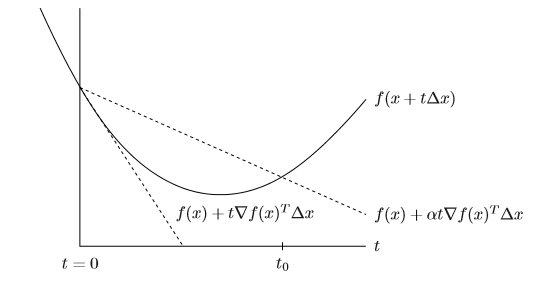
\includegraphics{fig9_1}
  \caption{\textit{Backtracking line search.} The backtracking condition is that $f$ lies below the upper dashed line, \ie $0\le t\le t_0$.}
  \label{fig:9.1}
\end{figure}
Note that we need to check $x+t\Delta x\in\dom f$ when using backtracking line search in practical implementation since $f$ is infinite outside its domain by our convention.
Then we start to check whether the inequality $f(x+t\Delta x)\le f(x)+\alpha t\nabla f(x)^T\Delta x$ holds.\par
The parameter $\alpha$ is typically chosen between $0.01$ and $0.3$, meaning that we accept a decrease in $f$ between $1\%$ and $30\%$ of the prediction based on the linear extrapolation.
The parameter $\beta$ is often chosen to be between $0.1$ (very crude search) and $0.8$ (less crude search).

% 9.3
\section{Gradient descent method}
Choose $\Delta x=-\nabla f(x)$, then \textit{gradient algorithm} or \textit{gradient descent method} is
\begin{algorithm}[\textit{Gradient descent method}]
  $ $\\
  \textbf{given} a starting point $x\in\dom f$.\\
  \textbf{repeat}
  \begin{enumerate}
    \item $\Delta x:=-\nabla f(x)$.
    \item \textit{Line search.} Choose step size $t$ via exact or backtracking line search.
    \item \textit{Update.} $x:=x+t\Delta x$
  \end{enumerate}
  \textbf{until} stopping criterion is satisfied.
\end{algorithm}
The criterion is usually $\|\nabla f(x)\|_2\le\eta$ where $\eta>0$ is small, and the condition is checked after step $1$ in most implementations.

% 9.3.1
\subsection{Convergence analysis}
\textcolor{red}{\textbf{Add in the future!}}

% 9.3.2
\subsection{Examples}
\subsubsection{A quadratic problem in $\R^2$}
Consider minimizing $f(x)=\frac{1}{2}(x_1^2+\gamma x_2^2)$ where $\gamma>0$.

\subsubsection{A nonquadratic problem in $\R^2$}
\subsubsection{A problem in $\R^{100}$}
\subsubsection{Gradient method and condition number}
\subsubsection{Conclusions}

% 9.4
\section{Steepest descent method}
\textcolor{red}{\textbf{Add in the future!}}

% 9.4.1
\subsection{Steepest descent for Euclidean and quadratic norms}
\subsubsection{Steepest descent for Euclidean norm}
\subsubsection{Steepest descent for quadratic norm}
\subsubsection{Interpretation via change of coordinates}

% 9.4.2
\subsection{Steepest descent for $\ell_1$-norm}

% 9.4.3
\subsection{Convergence analysis}

% 9.4.4
\subsection{Discussion and examples}
\subsubsection{Choice of norm for steepest descent}
\subsubsection{Examples}

% 9.5
\section{Newton's method}

% 9.5.1
\subsection{The Newton step}
The \textit{Newton step} is
\begin{align*}
  \Delta x_{nt}=-\nabla^2f(x)^{-1}\nabla f(x)
\end{align*}
Positive definiteness of $\nabla^2f(x)$ implies that
\begin{align*}
  \nabla f(x)^T\Delta x_{nt}=-\nabla f(x)^T\nabla^2f(x)^{-1}\nabla f(x)<0
\end{align*}
unless $\nabla f(x)=0$, so the Newton step is a descent direction.\\
The Newton step can be interpreted and motivated in several ways.

\subsubsection{Minimizer of second-order approximation}
The second-order Taylor approximation $\hat{f}$ of $f$ at $x$ is
\begin{align}
  \hat{f}(x+v)=f(x)+\nabla f(x)^Tv+\frac{1}{2}v^T\nabla^2 f(x)v\label{eq:9.28}
\end{align}
which is a convex quadratic function of $v$, and is minimized when $v=\Delta x_{nt}$.
Thus, $\Delta x_{nt}$ must be added to the point $x$ to minimize the second-order approximation of $f$ at $x$ as illustrated in figure \ref{fig:9.16}.
\begin{figure}
  \centering
  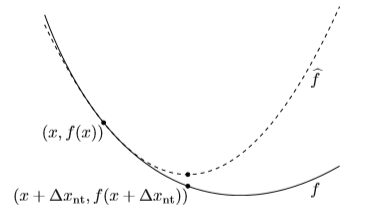
\includegraphics{fig9_16}
  \caption{The function $f$ and its second-order approximation $\hat{f}$.}
  \label{fig:9.16}
\end{figure}
The insights of Newton step are
\begin{itemize}
  \item if $f$ is quadratic, then $x+\Delta x_{nt}$ is the exact minimizer of $f$
  \item if $f$ is nearly quadratic, then $x+\Delta x_{nt}$ is a good estimate of the minimizer of $f$
  \item if $x$ is near $x^\ast$, then $x+\Delta x_{nt}$ is a good estimate of $x^\ast$
\end{itemize}

\subsubsection{Steepest descent direction in Hessian norm}
\textcolor{red}{\textbf{Add in the future!}}

\subsubsection{Solution of linearized optimality condition}
\textcolor{red}{\textbf{Add in the future!}}

\subsubsection{Affine invariance of the Newton step}
The Newton step is independent of linear (or affine) changes of coordinates.
Let $T\in\R^{n\times n}$ is nonsingular and $\bar{f}(y)=f(Ty)$, we have
\begin{align*}
  \nabla\bar{f}(y)=T^T\nabla f(x),\quad\nabla\bar{f}(y)=T^T\nabla^2f(x)T
\end{align*}
where $x=Ty$. The Newton step for $\bar{f}$ at $y$ is
\begin{align*}
  \Delta y_{nt} &= -(T^T\nabla^2f(x)T)^{-1}(T^T\nabla f(x))\\
                &= -T^{-1}\nabla^2f(x)^{-1}\nabla f(x)\\
                &= T^{-1}\Delta x_{nt}
\end{align*}
where $\Delta x_{nt}$ is the Newton step for $f$ at $x$, therefore $x+\Delta x_{nt}=T(y+\Delta y_{nt})$.

\subsubsection{The Newton decrement}
The \textit{Newton decrement} is
\begin{align*}
  \lambda(x)=(\nabla f(x)^T\nabla^2 f(x)^{-1}\nabla f(x))^{1/2}
\end{align*}
The relation between $f$ and the Newton decrement is
\begin{align*}
  f(x)-\inf_y\hat{f}(y)=f(x)-\hat{f}(x+\Delta x_{nt})=\frac{1}{2}\lambda(x)^2
\end{align*}
where $\hat{f}$ is the second-order approximation of $f$ at $x$.
\begin{itemize}
  \item $\lambda^2/2$ is an estimate of $f(x)-p^\ast$, based on the quadratic approximation of $f$ at $x$
  \item The Newton decrements can also expressed as
        \begin{align}
          \lambda(x)=(\Delta x_{nt}^T\nabla^2f(x)\Delta x_{nt})^{1/2}=\|\Delta x_{nt}\|_{\nabla^2f(x)}\label{eq:9.29}
        \end{align}
        this shows that $\lambda$ is the quadratic norm of the Newton step defined by Hessian $\nabla^2f(x)$.
  \item Using in backtracking line search, we have
        \begin{align}
          -\lambda(x)^2=\nabla f(x)^T\Delta x_{nt}=\frac{d}{dt}f(x+\Delta x_{nt}t)|_{t=0}\label{eq:9.30}
        \end{align}
        this constant can be interpreted as the directional derivative of $f$ at $x$ in the direction of the Newton step.
  \item Newton decrement is, like the Newton step, affine invariant, \ie the Newton decrement of $\bar{f}(y)=f(Ty)$ at $y$ is the same as the Newton decrement of $f$ at $x=Ty$ provided $T$ is nonsinngular.
\end{itemize}

% 9.5.2
\subsection{Newton's method}
The \textit{damped/guarded} Newton method is outlined below, and the \textit{pure} Newton method is to fix step size $t=1$.
\begin{algorithm}[\textit{Newton's method}]
  $ $\\
  \textbf{given} a starting point $x\in\dom f$, tolerance $\epsilon>0$.\\
  \textbf{repeat}
  \begin{enumerate}
    \item \textit{Compute the Newton step and decrement.}
      \begin{align*}
        \Delta x_{\text{nt}}:=-\nabla^2f(x)^{-1}\nabla f(x),\quad\lambda^2:=\nabla f(x)^T\nabla^2f(x)^{-1}\nabla f(x)
      \end{align*}
    \item \textit{Stopping criterion.} \textbf{quit} if $\lambda^2/2\le\epsilon$
    \item \textit{Line search.} Use backtracking line search.
    \item \textit{Update.} $x:=x+t\Delta x_{\text{nt}}$
  \end{enumerate}
\end{algorithm}
The minor difference from descent method is the position of the stopping criterion.

% 9.5.3
\subsection{Convergence analysis}

% 9.5.4
\subsection{Examples}

% 9.6
\section{Self-concordance}

% 9.7
\section{Implementation}
